As a fundamental building block of  modern computing systems, it is important for main memory to achieve short latency, high density, efficient energy and low cost, etc. Owing to the perfect balance on these aspects,  dynamic random access memory (DRAM) has been the de facto standard in the past few decades, and is widely deployed in almost all systems, including servers, desktops, mobile devices and embedded systems. 
And, whereas a bunch alternative memories have been proposed, such as PCM \cite{ISCA09:pcm}, STT-RAM \cite{ISPASS13:stt} and 3D-XPoint \cite{SOSP15:xpoint}, none of them is strictly superior to DRAM, and thus DRAM is unlikely to be completely replaced.
%And, DRAM is estimated to hold its status for a long time \cite{ISCA13:archshield, BOOK15:scaling}, though a bunch of alternative memories have been proposed, such as PCM \cite{ISCA09:pcm}, STT-RAM \cite{ISPASS13:stt} and 3D-XPoint \cite{SOSP15:xpoint}. 
DRAM's great success is tremendously contributed by its continuous technology scaling 
%from early above-100nm to nowadays 2x-nm 
to maintain performance growth and capacity enhancement. With the increasing stresses on capacity, bandwidth and performance from new high-performance applications and systems, DRAM must keep scaling down to meet the demands.

Unfortunately, scaling has become difficult due to the challenges to further shrink sizes of DRAM circuits and devices \cite{IBM02:scaling, IEDM10:scaling, MEMSYS15:twr}. 
As a result, memory accesses tends to take longer time to finish \cite{PATENT14:twr, PATENT15:twr}, cell behaviors are expected to be more statistical \cite{MEMSYS15:twr} and stored data is more vulnerable to disturbance and noise \cite{ISCA14:disturbance, DSN15:avatar, MEM14:twr}.
%On one hand, timing parameters become larger in smaller technology nodes \cite{PATENT14:twr, PATENT15:twr};
%on the other hand, it is more challenging to precisely control the fabrication process for finer node, and thus DRAM cell behaviors are expected to be more statistical than deterministic.
Consequently, many cells will violate the timing standards, and DRAM chip yield and reliability will be degraded, which is undesirable for the already tight profit margin of DRAM manufacturing. 

To mitigate the performance loss and yield degradation in further scaling, we need to expose the scaling effect to higher levels such that more effective approaches can be achieved with better trade-offs.  Candidate solutions can be proposed from multiple levels, ranging from devices to architectures and even to applications. And, the efficient ones require the cooperation from different components, including DRAM chips, memory controllers, operating systems and processors, etc.

\section{Problem Statement}
Scaling-down has been the conventionally effective method to grow DRAM chip capacity, to reduce power consumption and to lower the per-bit cost.
As scaling down, DRAM cells have been shrinking to smaller dimensions, which results in size reduction of access transistor, storage capacitor and peripheral circuits.
Firstly, smaller capacitor translates into a lower capacitance, reducing the stored charge; secondly, scaled DRAMs applies lower supply voltage \cite{ISCA13:ddr4, HPCA16:twr}, which further decreases per-cell charge and also increases the gate induced drain leakage \cite{ISCA13:archshield}; meanwhile, at smaller dimensions, adjacent cells are likely to electrically disturb each other \cite{ISCA14:disturbance};
moreover, smaller cell geometry increases the resistance on both access transistor and bitline \cite{ISCA13:ddr4, PATENT15:twr}, obstructing the cell charging process.
In addition to charge decrease, the input offset voltage on the sense amplifiers is also expected to increase \cite{HPCA16:twr, ISCA13:ddr4}, which makes it more difficult to sense data.

Moreover, scaling to smaller technology nodes grow the fabrication complexity and makes it more difficult to precisely control the dimensions of DRAM cells, which introduces more severe process variations (PV). Accordingly, DRAM cells are expected to show more statistical behaviors in a wide range; and, such uncertainty might cause increasingly more cells to violate the design specifications, which is beyond the tolerance of existing mechanisms such as row/column redundancy and ECC \cite{ISCA13:archshield}. 
As a result, a large number of chips would fail the testings.

The above phenomena of reduced dimensions and increased variability together adversely affect the data retention time, charge restoration and voltage sensing, which impact DRAM performance, reliability and cost from several aspects: (i) lower stored charge and higher leakage current introduces more leaky cells, which leads to more frequent refresh operations that harms performance, energy and reliability; (ii) slower charging process means longer restoring operation and potentially failing the standard specifications, which could hurt both performance and yield; (iii)  sensing difficulty lengthens the normal read/write accesses, and might cause access failures; (iv) close proximity of cells leads to electrical coupling effects, which might cause data to be faulty.

To tackle the scaling issues, whereas significant researches have been put into retention and refresh \cite{ED98:ret_dist, ITC08:ret_dist, EDL09:ret, MICRO10:smart_refresh, MICRO10:elastic_refresh, ISCA12:raidr, ISCA13:ret, ISCA13:ddr4,ISCA13:archshield, HPCA13:refresh_pausing, HPCA14:mosaic, SIGMETRICS14:vrt, DSN15:vrt, ISCA15:reflex} and sensing \cite{ISCA13:charm, HPCA13:tldram, HPCA14:nuat, HPCA15:al-dram}, restoring has not been paid attention to until recently and very few explorations \cite{MEM14:twr, ISCA15:mcr} have been performed.

%Naive solution to relax timing constraints, leading to serious performance degradation.
%Figure xxx.

%\section{Related Work}
%While write recovery time (tWR) keeps at 15ns across all generations \cite{JEDEC:ddr, JEDEC:ddr2, JEDEC:ddr3, JEDEC:ddr4}, it has to be lengthened in deep sub-micron technology nodes, which was first recently discussed by \citeN{MEM14:twr}.
%As the first academic work on tWR issues in further scaling DRAM, our paper \cite{DATE15:twr} studied the variation behaviors and proposed to utilize chunk remapping to lower restoration durations.
%Afterwards, patents on tWR were granted: \citeN{PATENT14:twr} raised the idea to adjust timings with respect to temperature, and \citeN{PATENT15:twr} claimed that tWR can be increased from 15ns to 60ns, and then explored backward compatibility.

%Whereas the tWR scaling issue has been identified in industrials, little academic research have been performed. Restoration has been a omitted issue util recently; people started to utilize the reserved timing margins \cite{DATE14:margin, HPCA15:al-dram}, with restoring being included. Besides, later work \cite{ISCA15:mcr} took use of charge variation to relax some timing constraints. However, none of these work targets at future DRAM technologies.

\section{Research Overview}
In this thesis, our research objective is explore the restoring operation in further scaling DRAM, and propose schemes to mitigate the induced issues like performance loss, yield degradation and other potential ones.
Specifically, this thesis plans to answer the following questions: 
%(i) how to utilize models and simulations to study the further scaling issues? 
(i) how to solve the enlarged timing constraints utilizing the memory organization characteristics? (ii) can we integrate the restoring with other memory operations to find solutions? (ii) what kind of help can we get from operating system and the applications?
Generally, this thesis tries to explore DRAM scaling from restoring perspective on different layers shown in Figure \ref{fig:thesis_work}, covering hardware architecture \ding{202}, operating system \ding{203} and applications \ding{204}, etc.

%\subsection{Framework to Study Restore Issues (Completed)}
%Modeling and simulation are required to perform the studies on further scaling DRAM.On device level, the models need to capture the critical components including transistor, capacitor and peripheral circuits; and the model should also cover the primary parameters and dimensions, such as transistor length/width, capacitance and voltage, etc. Further, to involve process variation effects, the models should be inherently statistical following certain distributions.

%With the constructed models, then we can move to chip generation, and then form ranks and DIMMs using the pool of chips. Next, architectural explorations can be conducted on the collected memory system. To get close to real manufacturing process, it is necessary to guarantee the quantities of chips, ranks and DIMMs large enough to be swept over in simulations.

\subsection{Achieve Fast Rows via Reorganization (Completed)}
Conventionally, a single set of timing constraints is applied to the whole memory system, which becomes undesirable in smaller feature size, because of the enlarged worst-case timing values. To preserve high chip yield, we should relax the timings to allow cells reliably finishing operations, which indicates a longer bank occupancy and thus degraded performance.


\begin{figure}
 \centering
    	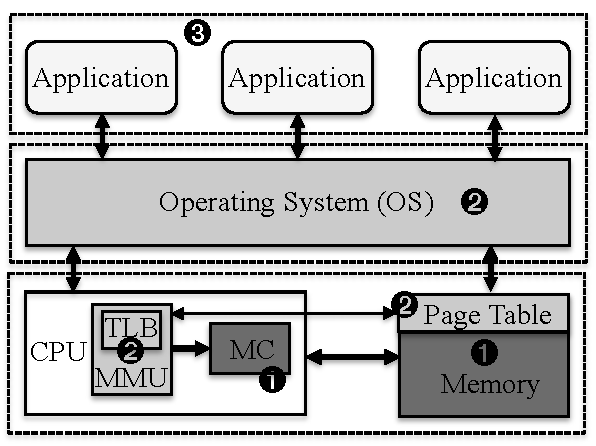
\includegraphics[width=0.4\linewidth]{figures/thesis_work.pdf}\\
  \vspace{-0.15in}
  \caption{Overall view of thesis work. While placing a focus on memory structures, we explore restoring effects from other layers, including page translation from operating system and inherent behaviors of applications.}
  \label{fig:thesis_work}
  \vspace{-0.45in}
\end{figure}

Fortunately, the variation characteristics also provide a large portion of good cells, which can be potentially utilized to compensate the bad ones.
Without modifying the DRAM cell structure, we can choose to expose the timing variations to architectural level. The memory controller can thus be enhanced to be variation-aware to compensate the performance loss.
The exploration can be performed either on coarse chip-level or fine chunk-level, depending the overhead budget and improvement goals.

Nevertheless, given the facts that each DRAM logical row is physically composed of multiple rows from different chips, and each chip row consists of thousands of cells, naively exposing timing is likely to offer very limited help. Accordingly, we choose to form logical rows by clustering similar fine-granularity chunks from different chips.
As a result, more fast memory regions can be exposed. 
In addition, we extend the idea to assembly phase, where compatible chips are grouped together to form ranks, and hence bad chip contamination could be well controlled.

From processor perspective, the aforementioned variation exploration provides non-uniform memory access (NUMA) characteristics, which can be utilized by operating system to speed up program execution.
Following the idea, we profile workloads to identify hot pages, and then allocate them to fast memory regions to maximize performance gains.

\subsection{Refresh-aware Partial Restore (Completed)}
Normal read/write accesses restore charge into cell capacitors to store data values. Due to DRAM's intrinsic leakage, the charge leaks over time, causing the stored data to be lost. To prevent this, periodical refreshes are required to recharge the cells. Given that cell voltage monotonically reduces between two refreshes and each refresh always fully charge the cells, full charge is unnecessary if the access is close in time to the next refresh.
 
The observation motivates us to propose refresh-distance-aware partial restore.
Restore operation is performed with respect to the distance to the coming refresh, and the closer to next refresh, the less charge is needed and thus the earlier the restore operation can be terminated. The idea is implemented by partitioning one refresh window (usually 64ms) into multiple sub-windows, and set different restoring goals, i.e., different timings, for each.

Whereas DRAM necessities frequent fresh to avoid data loss, the vast majority of cells can hold the data for much longer time, which inspires designs of multiple rate refresh \cite{EDL09:ret, ISCA12:raidr, ISCA15:reflex}.
Compared to refresh operations, restore contributes more critically to access latency and overall performance, and hence we might achieve more truncation opportunities by upgrading refresh rate. 
However, blind upgrading introduces more refreshes, which not only prolongs memory unavailable period but also consumes more energy.
As a compromise, we upgrade the refresh rate of selected bins, those were recently touched, and thus incur modest refreshing overhead to the system.

\subsection{Explore Restoring in Extended Scenarios (Future)}

\textbf{Approximate Computing:} While much performance loss in further scaling DRAMs can be recouped with the help of the proposed memory designs and the operating system, this might be over qualified for nowadays popular applications in domains like computer vision, machine learning and big data analytics.
%Those applications have intrinsic tolerance to inaccuracy; for example, many machine learning solutions are naturally imprecise by relying on heuristics to obtain acceptable results; and large-scale data analytics focus on aggregate trends rather the integrity of individual data elements. 
Those applications have intrinsic resilience to inaccuracy, which
provides a good opportunity to tolerate the slow-to-restore cells in memory. By annotating the approximate data \cite{PLDI11:enerj, MICRO13:appro, MICRO14:appro, MICRO15:doppelganger} which is tolerable to accuracy loss, we can shorten the restoring time of mapped memory locations. To guarantee the final output quality, we apply architectural techniques like error-correction and address remapping to avoid the faults of significant bits. Overall, we can achieve performance improvement and energy savings with a moderate sacrifice on output accuracy.

\textbf{Information leakage:} 
%Privacy, security and trust issues are rising concerns in modern computer systems, especially in cloud computing systems \cite{CLOUDCOM10:privacy}.
%Resource sharing and colocation of untrusted applications further worsen the situation by providing opportunities of timing-channel attacks \cite{HPCA14:channel, MICRO15:fs}.
Sensitive information leakage through memory access patterns are rising concerns, and a bunch of works \cite{CCS13:oram, HPCA14:channel, MICRO15:fs} have proposed to conceal the pattern.
And, things become more challenging when we consider approximate computing and restoring variations. While the former provides a new kind of side channel that allows attackers to correlate approximate data to its location origin \cite{ISCA15:prob}, the latter, even without approximate computing, is risky to leak more information on access patterns than prior cases \cite{HPCA14:channel, MICRO15:fs}, such as the possible physically mapped regions and the location correlation of accesses.

\textbf{3D-stacked and Temperature:}
Recent advances in die stacking techniques enables efficient integration of logic and memory dies in a single package, with a concrete example of Hybrid Memory Cube \cite{HMC:spec2}.
%HMC is especially promising for its innovative architecture that stacks multiple memory dies atop of the bottom logic die, and adopts packetized serial link interface to transfer data and requests \cite{ICCD15:dlb}.
%With the superior high bandwidth, low latency and packet-based interface, lots of work have proposed to move computation units inside the logic die \cite{JMicro:ndp, ISCA15:pim}.
However, thermal management is still a big issue in stacked memories \cite{DAC06:3dmodel, WONDP14:thermal}, and the deployment of bottom computation logics like simple cores \cite{ISCA15:pim} and even GPU \cite{HPDC14:pim_gpu} worsens the issue. Besides, temperature variations exist among vertical dies \cite{ICCD13:temp}. It is known that DRAM is sensitive to temperature changes, including refresh \cite{HPCA15:al-dram, ISCA13:ddr4} and restoring time \cite{PATENT14:twr, MEM14:twr}.
Therefore, it is worthwhile to explore restoring time in stacked memories, and utilize the temperature characteristics to dig more opportunities to boost performance. 

%\subsection{Combine tWR with Approximate Computing (Partially Completed)}
%\subsection{Study Security Issues of tWR Variation (Future)}
%\subsection{Explore tWR in 3D Stacked DRAM (Future)}

\section{Contributions}
This thesis makes the following contributions:

\begin{itemize}
\item We perform pioneering study on DRAM restoring in deep sub-micron scaling. We built models to simulate restoring behaviors and then generate DRAM devices to faithfully repeat the manufacturing process  and perform architectural-level studies.
\item Targeting at restoring issues, we propose schemes from different perspectives. On device and architectural levels, we apply chunk remapping and chip clustering techniques to achieve fast memory access; on system level, we maximizing performance improvement by allocating hot pages of the running workloads to fast regions.
\item Going further, we integrate restoring variation characteristics with approximate computing to strike a good balance among performance, energy and accuracy. We then explore restoring issues in extended scenarios including information leakage and 3D-stacked memory.  
\end{itemize}

%\section{THESIS STATEMENT}
%Defining a new sentiment analysis task (entity/event-level sentiment analysis task), this work develops annotated corpora as resources of the task and investigates joint prediction models integrating explicit sentiments, entity or event information and inference rules together to automatically recognize both explicit and implicit sentiments expressed among entities and events in the text.


\section{OUTLINE}
\label{outline}
The rest of this proposal is organized as follow:  
Chapter \ref{chapter:background} introduces the DRAM structures, operations and scaling issues.
In Chapter \ref{chapter:twr_reorganize}, we build models to study restoring effects, and then propose a series of techniques to shorten restoring timing values.
In Chapter \ref{chapter:partialrestore}, we explore the correlation between restoring and refresh, and seek the opportunities to early terminate restore operations.
Further restoring explorations are discussed in Chapter \ref{chapter:future_study}.
Chapter \ref{chapter:timeline} and \ref{chapter:summary} lists the timeline and concludes the proposal, respectively.








